\documentclass{beamer}
\usetheme[block=fill]{metropolis}
%\setbeamersize{text margin left=.2cm,text margin right=.2cm}
\usepackage{graphicx}
\graphicspath{{../../images/}}
%\usepackage[french]{babel}
%\usepackage{listings}
%\usepackage{lipsum}
\usepackage{boolexpr}
\usepackage{kpfonts}
\usepackage{caption}
\usepackage{wrapfig}
%\usepackage{chngcntr}
\usepackage[labelformat=empty]{caption}
\usepackage[official]{eurosym}

% http://tex.stackexchange.com/questions/114830/how-can-i-use-lvert-and-rvert-norm-symbols-x-with-the-iwona-math-font
\usepackage[math]{iwona}
\usepackage{scalerel}
\def\lVert{\mid\!\mid}
\def\rVert{\mid\!\mid}

\usepackage[normalem]{ulem}
%\newcommand{\Adj}{\mathbf{A}}
\usepackage{mathtools}

\usepackage{../../custom}
\usepackage{amsfonts}

%\usepackage[style=alphabetic,backend=bibtex]{biblatex}
%\addbibresource{../../biblio.bib}
%% See https://tex.stackexchange.com/questions/469555/unicode-u301-error-in-biblatex-but-not-in-main-text-i

\DeclareDatafieldSet{setall}{
  \member[datatype=literal]
  \member[datatype=name]
  \member[field=journal]% journal is special since it is
                        % actually journaltitle
}

\DeclareSourcemap{
  \maps[datatype=bibtex]{
    \map[overwrite, foreach={setall}]{
      % \`{\i}
      \step[fieldsource=\regexp{$MAPLOOP},
            match=\regexp{\x{0131}\x{0300}},
            replace=\regexp{\x{00EC}}]
      % \'{\i}
      \step[fieldsource=\regexp{$MAPLOOP},
            match=\regexp{\x{0131}\x{0301}},
            replace=\regexp{\x{00ED}}]
      % \^{\i}
      \step[fieldsource=\regexp{$MAPLOOP},
            match=\regexp{\x{0131}\x{0302}},
            replace=\regexp{\x{00EE}}]
      % \"{\i}
      \step[fieldsource=\regexp{$MAPLOOP},
            match=\regexp{\x{0131}\x{0308}},
            replace=\regexp{\x{00EF}}]
    }
  }
}




\usepackage{tikz}
\usetikzlibrary{arrows,matrix,decorations.pathreplacing,positioning,chains,fit,shapes,calc,3d}
\tikzset{box/.style={rectangle, draw=black, fill=black!8, align=center, rounded corners}}
\tikzset{function/.style={rectangle, draw=aurore, fill=aurore!8, align=center, rounded corners}}
\tikzset{solver/.style={rectangle, draw=canard, fill=canard!8, align=center, rounded corners}}
\tikzset{optimizer/.style={rectangle, draw=frambo, fill=frambo!8, align=center, rounded corners}}
\tikzset{alg/.style={rectangle, draw=lichen, fill=lichen!8, align=center, rounded corners}}
\tikzset{pkg/.style={rectangle, draw=black, fill=black!8, align=center, rounded corners}}

% Citations in footnote
% https://tex.stackexchange.com/a/29931/38244

\newcommand{\autocite}[1]{}
\newcommand{\footpartcite}[1]{}
%\DeclareCiteCommand{\footpartcite}[\mkbibfootnote]
%{\usebibmacro{prenote}}%
%{\usebibmacro{citeindex}%
%\tiny
%%\begin{spacing}{3}
%    \mkbibbrackets{\usebibmacro{cite}}%
%    \setunit{\addnbspace}
%    \printnames{labelname}%
%    \setunit{\labelnamepunct}
%    \printfield[citetitle]{title}%
%    \newunit
%    \printfield[]{year}}
%{\addsemicolon\space}
%{\usebibmacro{postnote}}
%
%\setbeamertemplate{footnote}{\insertfootnotetext}

\usepackage{framed}

%\usepackage{mathtools,xparse}
%\DeclarePairedDelimiter{\norm}{\lVert}{\rVert}
\newcommand\Wider[2][3em]{%
\makebox[\linewidth][c]{%
  \begin{minipage}{\dimexpr\textwidth+#1\relax}
  \raggedright#2
  \end{minipage}%
  }%
}

\title{Polynomial Optimization}
\date{July 28th, 2023}
\author{Beno\^it Legat}
\institute{
  \begin{minipage}{\textwidth}
    ERC ``Back to the Roots'' with Prof. Bart De Moor, STADIUS, KU Leuven

    \vspace{4em}
    
    \hfill\includegraphics[width=0.15\textwidth]{jump.png}-dev workshop 2023
  \end{minipage}
}
%\institute{JuMP-dev 2023}

% https://tex.stackexchange.com/questions/426088/texlive-pretest-2018-beamer-and-subfig-collide
\makeatletter
\let\@@magyar@captionfix\relax
\makeatother

\begin{document}
  \maketitle

\begin{frame}{Polynomial optimization}
  \vspace{-1em}
  \begin{align*}
    \min_{x \in \mathbb{R}^n} \quad & p(x)\\
    \text{s.t.} \quad & h_i(x) = 0 & \forall i \in \{1, \ldots, m_h\}\\
                \quad & g_i(x) \le 0 & \forall i \in \{1, \ldots, m_g\}\\
  \end{align*}
  where $p, h_i, g_i$ are \alert{polynomials}.
  
  \begin{block}{Easy or hard ?}
    \begin{itemize}
      \item In general, \alert{NP-hard}
      \item If $p, g_i$ are convex and $h_i$ are linear, it is convex...
      \item ... but in general, it is \alert{NP-hard}
      \item Special case with $p = 0$ and $m_g = 0$,
        system of polynomial equation, already \alert{NP-hard}...
    \end{itemize}
  \end{block}
\end{frame}

\begin{frame}{Two types of Lagrangian multipliers}
  \begin{block}{\alert{Constant} multipliers -- \alert{local} certificate -- KKT system}
    Find $x \in \R^n, \lambda \in \R^{m_h}, \sigma \in \R^{m_g}$ s.t.
    \[
      p(x) + \sum_{i=1}^{m_h} \lambda_i h_i(x) + \sum_{i=1}^{m_g} \sigma_i^2 g_i(x) = 0
    \]
  \end{block}
%  \begin{block}{\alert{Polynomial} multipliers -- \alert{global} certificate -- Positivstellensatz}
%    Find $k \in \mathbb{N}$, $\gamma \in \R$ and polynomials $\lambda_i(x) \in \R[x], s_i \in \preorder(g_1, \ldots, g_{m_g})$ s.t.
%    \[
%      s_0(p - \gamma) + \sum_{i=1}^{m_h} \lambda(x) h_i(x) + s_1 = (p - \gamma)^k
%    \]
%  \end{block}
  \begin{block}{\alert{Polynomial} multipliers -- \alert{global} certificate -- Putinar}
    Find $\gamma \in \R$ and polynomials $\lambda_i(x), \sigma_{i, j}(x) \in \R[x]$ s.t.
    \[
      p + \sum_{i=1}^{m_h} \lambda h_i + \sum_{i=1}^{m_g} \left(\sum_j \sigma_{i,j}^2\right) g_i = \gamma
    \]
  \end{block}
\end{frame}

\begin{frame}{Corner cases for KKT system}
  \begin{columns}
    \begin{column}{0.4\textwidth}
      \begin{align*}
        \min_{x \in \mathbb{R}^2} \quad & x + y\\
        \text{s.t.} \quad & (x + 1)^2 + y^2 \le 1\\
                          & (x - 1)^2 + y^2 \le 1\\
      \end{align*}
    \end{column}
    \begin{column}{0.4\textwidth}
      KKT system at $x = 0$:
      \begin{align*}
        1 + \sigma_1^2 - \sigma_2^2 & = 0 & \quad \partial/\partial x\\
        1 & = 0 & \quad \partial/\partial y
      \end{align*}
    \end{column}
  \end{columns}
  \vspace{-3em}
  \begin{center}
    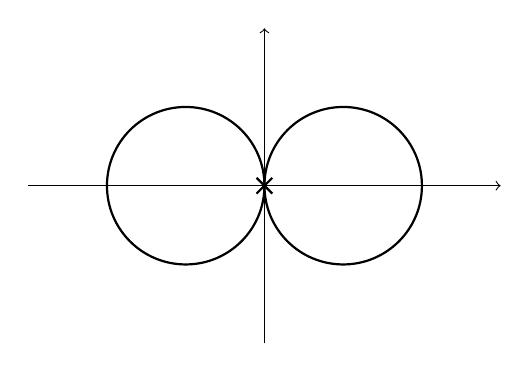
\begin{tikzpicture}
      \draw[->] (-3, 0) to (3, 0);
      \draw[->] (0, -2) to (0, 2);
      \draw[thick, -] (-0.1, -0.1) to (0.1, 0.1);
      \draw[thick, -] (-0.1, 0.1) to (0.1, -0.1);
      \draw[thick] (-1, 0) circle (1);
      \draw[thick] (1, 0) circle (1);
    \end{tikzpicture}
  \end{center}
  \begin{block}{What went wrong ?}
    \uncover<2>{
      The \alert{rank} of the jacobian dropped to \alert{1} at $x = 0$.
    }
  \end{block}
\end{frame}

\begin{frame}{Solving the KKT system}
  Given a system $S = \{\, x \mid h_i(x) = 0 \,\}$, for $i = 1, \ldots, m$,
  for any $\lambda \in \R[x]^m$,
  \[
    \sum_{i=1}^m \lambda_i(x) h_i(x) = 0, \qquad \forall x \in S.
  \]
  This is the linear span of,
  for all $\alpha \in \mathbb{N}^n, i \in \{1, \ldots, m\}$,
  \[
    x_1^{\alpha_1}x_2^{\alpha_2} \cdots x_n^{\alpha_n} h_i
  \]
  \emph{\alert{Macaulay} matrix} $M_d$ has these as rows if maxdegree below $d$.

  Buchberger : \alert{Gaussian elimination} $\to$ \alert{numerically unstable}!

  \begin{itemize}
    \item Let $Z_d$ be its right null space.
    \item \alert{Mind the gap} : rank of truncation of $Z_d$ equal to rank of $Z_d$
    \item Gap condition is \alert{sufficient} for finding the solution from $Z_d$.
  \end{itemize}
\end{frame}

\begin{frame}{Obtaining the minimizers for Sum-of-Squares}
  We search over \alert{dual} Lagrangian multipliers $\lambda_i(x)$, $\sigma_{i,j}(x)$.
  But then what's the \alert{primal} $x$ ? Isn't it the dual of the dual ?

  \begin{itemize}
    \item The \alert{conic dual} is a symmetric \alert{positive semidefinite} matrix of \alert{moments}.
    \item Positive semidefiniteness \alert{necessary} but not \alert{sufficient}
    for existence of a measure with these moments.
    \item \alert{Flatness property} : Rank of truncation equal to rank of full
    \item Flatness \alert{sufficient} condition for existence of an \alert{atomic}
    measure with these moments.
  \end{itemize}
\end{frame}

\begin{frame}{Polynomial Optimization Interface}
  \begin{center}
  \begin{tikzpicture}[scale = 0.9, every node/.style={scale=0.6}]
    \node[function] (SNF) at (0, 0) {\texttt{MOI.ScalarNonlinearFunction}};
    \node[solver] (LOC) at (-4, -2) {Local solver};
    \node[function] (SPF) at ( 4, -2) {\texttt{PolyJuMP.ScalarPolynomialFunction}};
    \node[function] (SQF) at (-4, -4) {\texttt{MOI.ScalarQuadraticFunction}};
    \node[optimizer] (SOS) at ( 0, -4) {\texttt{SumOfSquares.Optimizer}};
    \node[optimizer] (KKT) at ( 4, -4) {\texttt{PolyJuMP.KKT.Optimizer}};
    \node[solver] (QCQ) at (-4, -6) {QCQP solver};
    \node[solver] (CON) at ( 0, -6) {Conic solver};
    \node[alg] (ALG) at ( 4, -6) {\jlpkg{SemialgebraicSets} solver};
    \draw[thick, ->] (SNF.south west) to (LOC.north east);
    \draw[thick, ->] (SNF.south east) to (SPF.north);
    \draw[bend right=20, thick, ->] (SPF.west) to (SQF.north east);
    \draw[bend right=20, thick, ->] (SPF.south west) to (SOS.north);
    \draw[thick, ->] (SPF.south)      to (KKT.north);
    \draw[thick, ->] (SQF.south)      to (QCQ.north);
    \draw[thick, ->] (SOS.south)      to (CON.north);
    \draw[thick, ->] (KKT.south)      to (ALG.north);
  \end{tikzpicture}
  \end{center}
\end{frame}

\begin{frame}{Complementarity between Macaulay and Moment matrices}
  \Wider{
  \begin{center}
    \begin{tabular}{|l|c|c|}
      \hline
      & Moment matrix & Macaulay matrix\\
      \hline
      Relies on & \textcolor{lichen}{Conic solver} & \textcolor{lichen}{SVD}\\
      Fixed $d$ & \textcolor{lichen}{Polynomial} & \textcolor{lichen}{Polynomial}\\
      Growing $d$ & \textcolor{frambo}{Exponential} & \textcolor{frambo}{Exponential}\\
      & \textcolor{lichen}{Real radical} & \textcolor{frambo}{Spurious complex solutions}\\
      & \textcolor{lichen}{Complementary slackness} & \textcolor{frambo}{Spurious FOCPs}\\
      & \textcolor{frambo}{Low-accuracy system} & \textcolor{lichen}{Numerically robust}\\
      \hline
    \end{tabular}
  \end{center}
  \uncover<2>{Seems complementary, could they work together ?}
  }
\end{frame}

\begin{frame}{Mixing Macaulay and Sum-of-Squares frameworks}
  \begin{center}
  \begin{tikzpicture}[scale = 0.9, every node/.style={scale=0.6}]
    \node[box] (OPT) at (0, 2) {\begin{minipage}{6em}\centering Polynomial Optimization\end{minipage}};
    \node[box] (MacMat) at (3, 2) {\begin{minipage}{4em}\centering Macaulay Matrix\end{minipage}};
    \node[box] (MH) at (6, 2) {\begin{minipage}{4em}\centering Moment Matrix\end{minipage}};
    \node[box] (SYS) at (2, -2) {\begin{minipage}{5em}\centering Polynomial System\end{minipage}};
    \node[box] (NULL) at (4.5, 0) {\begin{minipage}{5em}\centering Macaulay Null space\end{minipage}};
    \node[box] (BB) at (7, -2) {\begin{minipage}{3em}\centering Border Basis\end{minipage}};
    \node[box] (SOL) at (10, -2) {Solutions};
    \node[box] (MUL) at (9, 2) {\begin{minipage}{6em}\centering Multiplication Matrix\end{minipage}};
    \draw[bend left=20, thick, ->] (OPT.north east) to node[above] {\jlpkg{SumOfSquares}} (MH.north west);
    \draw[thick, ->] (OPT.south east) to node[rotate=-83, below] {\jlpkg{PolyJuMP} -- KKT} (SYS.north west);
    \draw[color=canard, thick, ->] (MH.south west) to node[rotate=80, below] {Image~\autocite{lasserre2008semidefinite}} (NULL.north east);
    %\draw[thick, bend left=30, ->] (NULL.south west) to node[above=0.3em] {\alert{\textbf{Hankel}}} (MH.south east);
    %\draw[bend left=30, thick, ->] (SYS.north) to node[rotate = 90, above] {Sum-of-Squares~\autocite{lasserre2008semidefinite}\footpartcite{lasserre2008semidefinite}} (MH.south);
    %\draw[bend left=30, thick, ->] (MH.south) to node[rotate = 90, above]{SVD~\autocite{lasserre2008semidefinite}} (SYS.north);
    %\draw[bend left = -30, thick, ->] (NULL.south west) to node[above,rotate=65] {Lukas ?} (SYS.north east);
    \draw[color=frambo, thick, ->] (SYS.north) to
    %node[below,rotate=90] {Macaulay~\autocite{dreesen2012back}}
    (MacMat.south west);
    \draw[color=frambo, thick, ->] (MacMat.south east) to node[below,rotate=-83] {Kernel} (NULL.north west);
    %\draw[thick, ->] (NULL.south) to node[rotate=-90, above] {Row Echelon~\autocite{dreesen2012back}~\autocite{henrion2005detecting}\footpartcite{henrion2005detecting}} (BB.north);
    %\draw[bend left=30, thick, ->] (NULL.south) to (SYS.north east);
    %\draw[bend right=30, thick, ->] (NULL.south) to (BB.north west);
    \draw[color=canard, thick, -] (NULL.south) to (4.5, -1);
    \draw[color=canard, thick, ->] (4.5, -1) to (SYS.north east);
    \draw[color=canard, thick, ->] (4.5, -1) to (BB.north west);
    \draw[color=aurore, thick, ->] (SYS.east) to node[below] {\jlpkg{Groebner} -- Faug\`ere's F4} (BB.west);
    \draw[color=lichen, dashed, thick, ->] (SYS.east) to node[color=lichen, above] {Buchberger} (BB.west);
    \draw[color=canard, thick, -] (BB.north east) to (MUL.south west);
    \draw[color=lichen, dashed, thick, ->] (BB.north east) to (MUL.south west);
    \draw[color=canard, thick, ->] (MH.north east) to node[above] {Flatness} (MUL.north west);
    \draw[color=canard, thick, ->] (NULL.east) to node[rotate=35, below] {Mind the gap!} (MUL.west);
    %\draw[thick, ->] (NULL.south east) to node[rotate=-66, above] {Shift~\autocite{dreesen2012back}\footpartcite{dreesen2012back}} (MUL.north west);
    %\draw[bend right = 120, thick, ->] (NULL.east) to node[rotate=-25, above] {Lukas ?} (NULL.north);
    \draw[color=lichen, thick, ->] (MUL.south) to node[rotate=-70, below] {Schur~\autocite{corless1997reordered}\footpartcite{corless1997reordered}} (SOL.north);
    \draw[bend right = 10, thick, ->] (SYS.south) to node[below] {\jlpkg{HomotopyContinuation}} (SOL.south west);
    \node[pkg, dashed, color=canard, fill=canard!5] at (8, 3) {\jlpkg{MultivariateMoments}};
    \node[pkg, dashed, color=lichen, fill=lichen!5] at (9.2, -2.9) {\jlpkg{SemialgebraicSets}};
    \node[pkg, dashed, color=frambo, fill=frambo!5] at (1.2, -2.9) {\jlpkg{Macaulay}};
  \end{tikzpicture}
  \end{center}
\end{frame}

\end{document}
